\documentclass[15pt,a4paper]{article}
\usepackage[polish]{babel}
\usepackage[unicode]{hyperref}
\usepackage[MeX]{polski}
\usepackage[utf8]{inputenc}
\usepackage[T1]{fontenc}
\usepackage[top=2cm,bottom=2cm,left=2cm,right=2cm]{geometry}
\usepackage{enumerate}
\usepackage{graphicx}
\usepackage{bmpsize}
\title{Triki kuglarskie}
\author{Marta Kotewicz}
\date{}
\begin{document}

\maketitle
Do trików kuglarskich jest potrzebne dużo rzeczy. Sprzęt, umiejętności i wiele innych. Warto pamiętać, że przede wszystkim jest to świetna zabawa dla widza jak i dla artysty.\
Sprzęty w kuglarstwie można dzielić na te, które można podpalić i na te które, używa się wyłącznie "na sucho", czyli bez ognia. Niektóre z nich przedstawione są w tabelce poniżej:\
\begin{center}
\begin{tabular}{|c|r|}
\hline
Na sucho & Do ognia\\
\hline
\hline
akryle\footnote & poi\\
\hline
obręcze & kije\\
\hline
monocykle\footnote & wachlarze\\
\hline
chusty\footnote & pochodnie\\
\hline
\end{tabular}
\end{center}
\addtocounter{footnote}{-2}
\footnotetext{przezroczyste kule, które sprawiają wrażenie szklanych}
\stepcounter{footnote}
\footnotetext{rowery składające się z jednego koła}
\stepcounter{footnote}
\footnotetext{chusty używane do akrobatyki powietrznej}

\section{Co jest nam potrzebne do nauczenia się trików}
Jeśli chcemy się nauczyć czegoś fajnego musimy zwracać uwagę na wiele czynników, które okazują się być potrzebne do zrozumienia podstawy sztuczek.
 \subsection{W psychice}
\begin{itemize}
  \item Chęci
  \item Cierpliwość
  \item Zawziętość
\end{itemize}

\subsection{Fizycznie}
\begin{enumerate}
  \item Rozgrzewka
  \item Sprzęt
  \item Płaszczyzny \ldots
\end{enumerate}

\section{Płaszczyzny}
Płaszczyzny mają wielkie znaczenie, przy robieniu trików. Niekiedy bez zachowania odpowiednich płaszczyzn trik nam nie wyjdzie.
 \subsection{Wzór ogólny}
 \begin{equation}
 \textrm{W przestrzeni euklidesowej }
 R^3
 \end{equation} płaszczyzna jest zbiorem punktów, których współrzędne spełniają w danym kartezjańskim układzie współrzędnych równanie:
 \begin{equation}
 Ax+By+Cz+D=0\footnote{z postaci ogólnej wzoru można przejść do postaci normalnej}
 \end{equation}
przy czym liczby A, B, C, nie mogą być jednocześnie równe zeru.\
 \subsection{Wzór normalny}
 Równanie normalne płaszczyzny, to równanie postaci:
 \begin{equation}
 \alpha x + \beta y + \gamma z + \delta = 0\
 \end{equation} 
\begin{equation}
 \textrm{gdzie }
 \alpha^2 + \beta^2 + \gamma^2 = 1.
 \end{equation} 
 \begin{equation}\textrm{Liczby: } \alpha, \beta, \gamma 
 \end{equation}
  interpretujemy jako cosinusy kierunkowe prostej prostopadłej do płaszczyzny.

\begin{figure}
\centering
\graphicspath{{/projektLaTeXmkotewicz.s-/}}
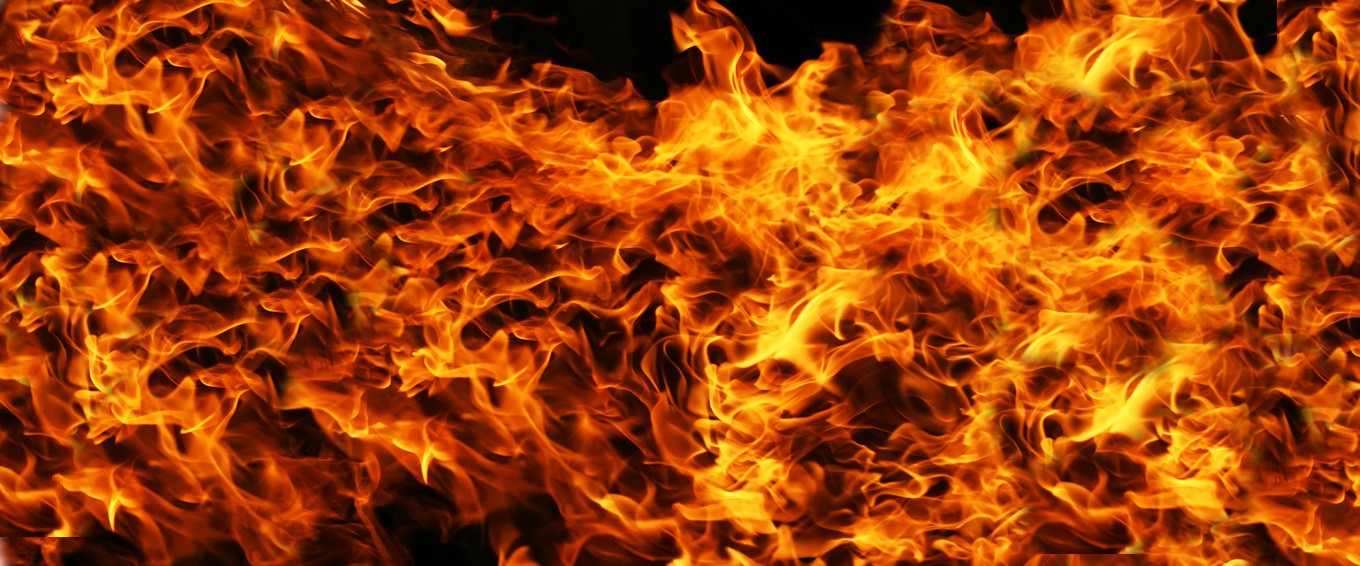
\includegraphics[scale=0.1,natwidth=1360,natheight=556]{ognia.jpg}
\caption{ognia}\label{rys:logo:jeden}
\end{figure}

\begin{thebibliography}{9}
\bibitem{ciocia}
  Ciocia Wikipedia,
  \emph{Płaszczyzna}.
\end{thebibliography}

\end{document}